
\documentclass[10pt]{article}
\usepackage{color}
\usepackage{makeidx}
\usepackage{graphicx}
\usepackage[section]{placeins}
\makeindex
\begin{document}
\begin{titlepage}
\centering
\huge{CMPE 315: Principles of VLSI Design Lab Cover Page}
\vfill
\flushleft
\large{
Lab \#: 2\\
Lab Title: Schematic Design and SpectreS Simulations\\}
\vfill
Name: Brian Weber\\
Section: CMPE640 01\\
\vfill
Date Submitted: 10/2/2017
\vfill
\Large{TA / Grader Use Only:}\\
Late Submission Deduction (20\% per day):\\
\vspace{1cm}
Other Deductions:\\
\vspace{3cm}
Final Lab Grade:\\
\vspace{1cm}
Comments to student:\\
\vspace{5cm}
\end{titlepage}
\tableofcontents
\begin{figure}[htb]
    \centering
    \begingroup
    \fontsize{8pt}{8pt}\selectfont
    % GNUPLOT: LaTeX picture with Postscript
\begingroup
  \makeatletter
  \providecommand\color[2][]{%
    \GenericError{(gnuplot) \space\space\space\@spaces}{%
      Package color not loaded in conjunction with
      terminal option `colourtext'%
    }{See the gnuplot documentation for explanation.%
    }{Either use 'blacktext' in gnuplot or load the package
      color.sty in LaTeX.}%
    \renewcommand\color[2][]{}%
  }%
  \providecommand\includegraphics[2][]{%
    \GenericError{(gnuplot) \space\space\space\@spaces}{%
      Package graphicx or graphics not loaded%
    }{See the gnuplot documentation for explanation.%
    }{The gnuplot epslatex terminal needs graphicx.sty or graphics.sty.}%
    \renewcommand\includegraphics[2][]{}%
  }%
  \providecommand\rotatebox[2]{#2}%
  \@ifundefined{ifGPcolor}{%
    \newif\ifGPcolor
    \GPcolortrue
  }{}%
  \@ifundefined{ifGPblacktext}{%
    \newif\ifGPblacktext
    \GPblacktextfalse
  }{}%
  % define a \g@addto@macro without @ in the name:
  \let\gplgaddtomacro\g@addto@macro
  % define empty templates for all commands taking text:
  \gdef\gplbacktext{}%
  \gdef\gplfronttext{}%
  \makeatother
  \ifGPblacktext
    % no textcolor at all
    \def\colorrgb#1{}%
    \def\colorgray#1{}%
  \else
    % gray or color?
    \ifGPcolor
      \def\colorrgb#1{\color[rgb]{#1}}%
      \def\colorgray#1{\color[gray]{#1}}%
      \expandafter\def\csname LTw\endcsname{\color{white}}%
      \expandafter\def\csname LTb\endcsname{\color{black}}%
      \expandafter\def\csname LTa\endcsname{\color{black}}%
      \expandafter\def\csname LT0\endcsname{\color[rgb]{1,0,0}}%
      \expandafter\def\csname LT1\endcsname{\color[rgb]{0,1,0}}%
      \expandafter\def\csname LT2\endcsname{\color[rgb]{0,0,1}}%
      \expandafter\def\csname LT3\endcsname{\color[rgb]{1,0,1}}%
      \expandafter\def\csname LT4\endcsname{\color[rgb]{0,1,1}}%
      \expandafter\def\csname LT5\endcsname{\color[rgb]{1,1,0}}%
      \expandafter\def\csname LT6\endcsname{\color[rgb]{0,0,0}}%
      \expandafter\def\csname LT7\endcsname{\color[rgb]{1,0.3,0}}%
      \expandafter\def\csname LT8\endcsname{\color[rgb]{0.5,0.5,0.5}}%
    \else
      % gray
      \def\colorrgb#1{\color{black}}%
      \def\colorgray#1{\color[gray]{#1}}%
      \expandafter\def\csname LTw\endcsname{\color{white}}%
      \expandafter\def\csname LTb\endcsname{\color{black}}%
      \expandafter\def\csname LTa\endcsname{\color{black}}%
      \expandafter\def\csname LT0\endcsname{\color{black}}%
      \expandafter\def\csname LT1\endcsname{\color{black}}%
      \expandafter\def\csname LT2\endcsname{\color{black}}%
      \expandafter\def\csname LT3\endcsname{\color{black}}%
      \expandafter\def\csname LT4\endcsname{\color{black}}%
      \expandafter\def\csname LT5\endcsname{\color{black}}%
      \expandafter\def\csname LT6\endcsname{\color{black}}%
      \expandafter\def\csname LT7\endcsname{\color{black}}%
      \expandafter\def\csname LT8\endcsname{\color{black}}%
    \fi
  \fi
    \setlength{\unitlength}{0.0500bp}%
    \ifx\gptboxheight\undefined%
      \newlength{\gptboxheight}%
      \newlength{\gptboxwidth}%
      \newsavebox{\gptboxtext}%
    \fi%
    \setlength{\fboxrule}{0.5pt}%
    \setlength{\fboxsep}{1pt}%
\begin{picture}(7200.00,5400.00)%
    \gplgaddtomacro\gplbacktext{%
      \csname LTb\endcsname%%
      \put(550,189){\makebox(0,0)[r]{\strut{}$0$}}%
      \put(550,890){\makebox(0,0)[r]{\strut{}$5$}}%
      \put(682,-220){\makebox(0,0){\strut{}$0$}}%
      \put(1447,-220){\makebox(0,0){\strut{}$1\times10^{-8}$}}%
      \put(2212,-220){\makebox(0,0){\strut{}$2\times10^{-8}$}}%
      \put(2977,-220){\makebox(0,0){\strut{}$3\times10^{-8}$}}%
      \put(3743,-220){\makebox(0,0){\strut{}$4\times10^{-8}$}}%
      \put(4508,-220){\makebox(0,0){\strut{}$5\times10^{-8}$}}%
      \put(5273,-220){\makebox(0,0){\strut{}$6\times10^{-8}$}}%
      \put(6038,-220){\makebox(0,0){\strut{}$7\times10^{-8}$}}%
      \put(6803,-220){\makebox(0,0){\strut{}$8\times10^{-8}$}}%
    }%
    \gplgaddtomacro\gplfronttext{%
      \csname LTb\endcsname%%
      \put(330,539){\rotatebox{-270}{\makebox(0,0){\strut{}D}}}%
    }%
    \gplgaddtomacro\gplbacktext{%
      \csname LTb\endcsname%%
      \put(550,1268){\makebox(0,0)[r]{\strut{}$0$}}%
      \put(550,1970){\makebox(0,0)[r]{\strut{}$5$}}%
      \put(682,859){\makebox(0,0){\strut{}}}%
      \put(1447,859){\makebox(0,0){\strut{}}}%
      \put(2212,859){\makebox(0,0){\strut{}}}%
      \put(2977,859){\makebox(0,0){\strut{}}}%
      \put(3743,859){\makebox(0,0){\strut{}}}%
      \put(4508,859){\makebox(0,0){\strut{}}}%
      \put(5273,859){\makebox(0,0){\strut{}}}%
      \put(6038,859){\makebox(0,0){\strut{}}}%
      \put(6803,859){\makebox(0,0){\strut{}}}%
    }%
    \gplgaddtomacro\gplfronttext{%
      \csname LTb\endcsname%%
      \put(330,1619){\rotatebox{-270}{\makebox(0,0){\strut{}C}}}%
    }%
    \gplgaddtomacro\gplbacktext{%
      \csname LTb\endcsname%%
      \put(550,2348){\makebox(0,0)[r]{\strut{}$0$}}%
      \put(550,3050){\makebox(0,0)[r]{\strut{}$5$}}%
      \put(682,1939){\makebox(0,0){\strut{}}}%
      \put(1447,1939){\makebox(0,0){\strut{}}}%
      \put(2212,1939){\makebox(0,0){\strut{}}}%
      \put(2977,1939){\makebox(0,0){\strut{}}}%
      \put(3743,1939){\makebox(0,0){\strut{}}}%
      \put(4508,1939){\makebox(0,0){\strut{}}}%
      \put(5273,1939){\makebox(0,0){\strut{}}}%
      \put(6038,1939){\makebox(0,0){\strut{}}}%
      \put(6803,1939){\makebox(0,0){\strut{}}}%
    }%
    \gplgaddtomacro\gplfronttext{%
      \csname LTb\endcsname%%
      \put(330,2699){\rotatebox{-270}{\makebox(0,0){\strut{}B}}}%
    }%
    \gplgaddtomacro\gplbacktext{%
      \csname LTb\endcsname%%
      \put(550,3429){\makebox(0,0)[r]{\strut{}$0$}}%
      \put(550,4130){\makebox(0,0)[r]{\strut{}$5$}}%
      \put(682,3020){\makebox(0,0){\strut{}}}%
      \put(1447,3020){\makebox(0,0){\strut{}}}%
      \put(2212,3020){\makebox(0,0){\strut{}}}%
      \put(2977,3020){\makebox(0,0){\strut{}}}%
      \put(3743,3020){\makebox(0,0){\strut{}}}%
      \put(4508,3020){\makebox(0,0){\strut{}}}%
      \put(5273,3020){\makebox(0,0){\strut{}}}%
      \put(6038,3020){\makebox(0,0){\strut{}}}%
      \put(6803,3020){\makebox(0,0){\strut{}}}%
    }%
    \gplgaddtomacro\gplfronttext{%
      \csname LTb\endcsname%%
      \put(330,3779){\rotatebox{-270}{\makebox(0,0){\strut{}A}}}%
    }%
    \gplgaddtomacro\gplbacktext{%
      \csname LTb\endcsname%%
      \put(550,4509){\makebox(0,0)[r]{\strut{}$0$}}%
      \put(550,5210){\makebox(0,0)[r]{\strut{}$5$}}%
      \put(682,4100){\makebox(0,0){\strut{}}}%
      \put(1447,4100){\makebox(0,0){\strut{}}}%
      \put(2212,4100){\makebox(0,0){\strut{}}}%
      \put(2977,4100){\makebox(0,0){\strut{}}}%
      \put(3743,4100){\makebox(0,0){\strut{}}}%
      \put(4508,4100){\makebox(0,0){\strut{}}}%
      \put(5273,4100){\makebox(0,0){\strut{}}}%
      \put(6038,4100){\makebox(0,0){\strut{}}}%
      \put(6803,4100){\makebox(0,0){\strut{}}}%
    }%
    \gplgaddtomacro\gplfronttext{%
      \csname LTb\endcsname%%
      \put(330,4859){\rotatebox{-270}{\makebox(0,0){\strut{}Out}}}%
      \put(3742,5729){\makebox(0,0){\strut{}AOI Extracted View Functionality Simulation}}%
    }%
    \gplbacktext
    \put(0,0){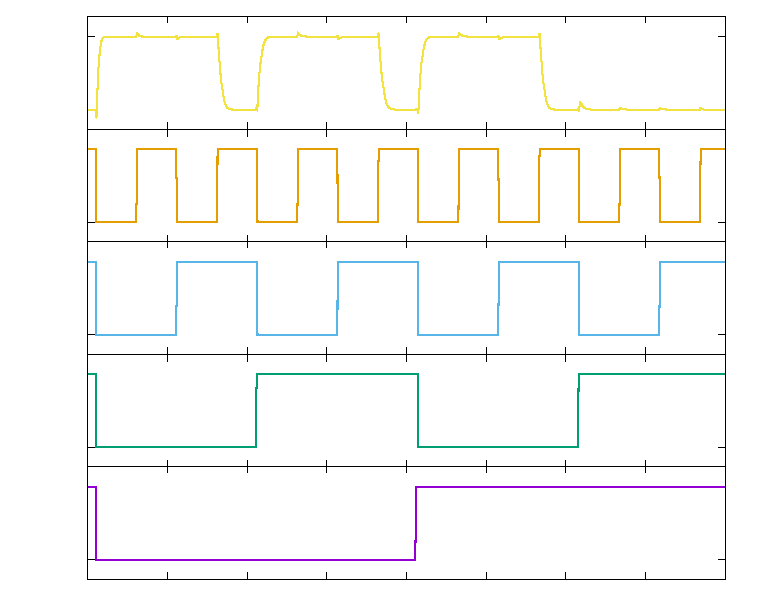
\includegraphics{aoi_func}}%
    \gplfronttext
  \end{picture}%
\endgroup

    \endgroup
    \caption{Waveform plots of the output of an X4 inverter driving different amounts of load inverters.}
    \label{aoi_func}
\end{figure}
\begin{figure}[htb]
    \centering
    \begingroup
    \fontsize{8pt}{8pt}\selectfont
    % GNUPLOT: LaTeX picture with Postscript
\begingroup
  \makeatletter
  \providecommand\color[2][]{%
    \GenericError{(gnuplot) \space\space\space\@spaces}{%
      Package color not loaded in conjunction with
      terminal option `colourtext'%
    }{See the gnuplot documentation for explanation.%
    }{Either use 'blacktext' in gnuplot or load the package
      color.sty in LaTeX.}%
    \renewcommand\color[2][]{}%
  }%
  \providecommand\includegraphics[2][]{%
    \GenericError{(gnuplot) \space\space\space\@spaces}{%
      Package graphicx or graphics not loaded%
    }{See the gnuplot documentation for explanation.%
    }{The gnuplot epslatex terminal needs graphicx.sty or graphics.sty.}%
    \renewcommand\includegraphics[2][]{}%
  }%
  \providecommand\rotatebox[2]{#2}%
  \@ifundefined{ifGPcolor}{%
    \newif\ifGPcolor
    \GPcolortrue
  }{}%
  \@ifundefined{ifGPblacktext}{%
    \newif\ifGPblacktext
    \GPblacktextfalse
  }{}%
  % define a \g@addto@macro without @ in the name:
  \let\gplgaddtomacro\g@addto@macro
  % define empty templates for all commands taking text:
  \gdef\gplbacktext{}%
  \gdef\gplfronttext{}%
  \makeatother
  \ifGPblacktext
    % no textcolor at all
    \def\colorrgb#1{}%
    \def\colorgray#1{}%
  \else
    % gray or color?
    \ifGPcolor
      \def\colorrgb#1{\color[rgb]{#1}}%
      \def\colorgray#1{\color[gray]{#1}}%
      \expandafter\def\csname LTw\endcsname{\color{white}}%
      \expandafter\def\csname LTb\endcsname{\color{black}}%
      \expandafter\def\csname LTa\endcsname{\color{black}}%
      \expandafter\def\csname LT0\endcsname{\color[rgb]{1,0,0}}%
      \expandafter\def\csname LT1\endcsname{\color[rgb]{0,1,0}}%
      \expandafter\def\csname LT2\endcsname{\color[rgb]{0,0,1}}%
      \expandafter\def\csname LT3\endcsname{\color[rgb]{1,0,1}}%
      \expandafter\def\csname LT4\endcsname{\color[rgb]{0,1,1}}%
      \expandafter\def\csname LT5\endcsname{\color[rgb]{1,1,0}}%
      \expandafter\def\csname LT6\endcsname{\color[rgb]{0,0,0}}%
      \expandafter\def\csname LT7\endcsname{\color[rgb]{1,0.3,0}}%
      \expandafter\def\csname LT8\endcsname{\color[rgb]{0.5,0.5,0.5}}%
    \else
      % gray
      \def\colorrgb#1{\color{black}}%
      \def\colorgray#1{\color[gray]{#1}}%
      \expandafter\def\csname LTw\endcsname{\color{white}}%
      \expandafter\def\csname LTb\endcsname{\color{black}}%
      \expandafter\def\csname LTa\endcsname{\color{black}}%
      \expandafter\def\csname LT0\endcsname{\color{black}}%
      \expandafter\def\csname LT1\endcsname{\color{black}}%
      \expandafter\def\csname LT2\endcsname{\color{black}}%
      \expandafter\def\csname LT3\endcsname{\color{black}}%
      \expandafter\def\csname LT4\endcsname{\color{black}}%
      \expandafter\def\csname LT5\endcsname{\color{black}}%
      \expandafter\def\csname LT6\endcsname{\color{black}}%
      \expandafter\def\csname LT7\endcsname{\color{black}}%
      \expandafter\def\csname LT8\endcsname{\color{black}}%
    \fi
  \fi
    \setlength{\unitlength}{0.0500bp}%
    \ifx\gptboxheight\undefined%
      \newlength{\gptboxheight}%
      \newlength{\gptboxwidth}%
      \newsavebox{\gptboxtext}%
    \fi%
    \setlength{\fboxrule}{0.5pt}%
    \setlength{\fboxsep}{1pt}%
\begin{picture}(7200.00,5400.00)%
    \gplgaddtomacro\gplbacktext{%
      \csname LTb\endcsname%%
      \put(550,189){\makebox(0,0)[r]{\strut{}$0$}}%
      \put(550,890){\makebox(0,0)[r]{\strut{}$5$}}%
      \put(682,-220){\makebox(0,0){\strut{}$0$}}%
      \put(1447,-220){\makebox(0,0){\strut{}$1\times10^{-8}$}}%
      \put(2212,-220){\makebox(0,0){\strut{}$2\times10^{-8}$}}%
      \put(2977,-220){\makebox(0,0){\strut{}$3\times10^{-8}$}}%
      \put(3743,-220){\makebox(0,0){\strut{}$4\times10^{-8}$}}%
      \put(4508,-220){\makebox(0,0){\strut{}$5\times10^{-8}$}}%
      \put(5273,-220){\makebox(0,0){\strut{}$6\times10^{-8}$}}%
      \put(6038,-220){\makebox(0,0){\strut{}$7\times10^{-8}$}}%
      \put(6803,-220){\makebox(0,0){\strut{}$8\times10^{-8}$}}%
    }%
    \gplgaddtomacro\gplfronttext{%
      \csname LTb\endcsname%%
      \put(330,539){\rotatebox{-270}{\makebox(0,0){\strut{}D}}}%
    }%
    \gplgaddtomacro\gplbacktext{%
      \csname LTb\endcsname%%
      \put(550,1268){\makebox(0,0)[r]{\strut{}$0$}}%
      \put(550,1970){\makebox(0,0)[r]{\strut{}$5$}}%
      \put(682,859){\makebox(0,0){\strut{}}}%
      \put(1447,859){\makebox(0,0){\strut{}}}%
      \put(2212,859){\makebox(0,0){\strut{}}}%
      \put(2977,859){\makebox(0,0){\strut{}}}%
      \put(3743,859){\makebox(0,0){\strut{}}}%
      \put(4508,859){\makebox(0,0){\strut{}}}%
      \put(5273,859){\makebox(0,0){\strut{}}}%
      \put(6038,859){\makebox(0,0){\strut{}}}%
      \put(6803,859){\makebox(0,0){\strut{}}}%
    }%
    \gplgaddtomacro\gplfronttext{%
      \csname LTb\endcsname%%
      \put(330,1619){\rotatebox{-270}{\makebox(0,0){\strut{}C}}}%
    }%
    \gplgaddtomacro\gplbacktext{%
      \csname LTb\endcsname%%
      \put(550,2348){\makebox(0,0)[r]{\strut{}$0$}}%
      \put(550,3050){\makebox(0,0)[r]{\strut{}$5$}}%
      \put(682,1939){\makebox(0,0){\strut{}}}%
      \put(1447,1939){\makebox(0,0){\strut{}}}%
      \put(2212,1939){\makebox(0,0){\strut{}}}%
      \put(2977,1939){\makebox(0,0){\strut{}}}%
      \put(3743,1939){\makebox(0,0){\strut{}}}%
      \put(4508,1939){\makebox(0,0){\strut{}}}%
      \put(5273,1939){\makebox(0,0){\strut{}}}%
      \put(6038,1939){\makebox(0,0){\strut{}}}%
      \put(6803,1939){\makebox(0,0){\strut{}}}%
    }%
    \gplgaddtomacro\gplfronttext{%
      \csname LTb\endcsname%%
      \put(330,2699){\rotatebox{-270}{\makebox(0,0){\strut{}B}}}%
    }%
    \gplgaddtomacro\gplbacktext{%
      \csname LTb\endcsname%%
      \put(550,3429){\makebox(0,0)[r]{\strut{}$0$}}%
      \put(550,4130){\makebox(0,0)[r]{\strut{}$5$}}%
      \put(682,3020){\makebox(0,0){\strut{}}}%
      \put(1447,3020){\makebox(0,0){\strut{}}}%
      \put(2212,3020){\makebox(0,0){\strut{}}}%
      \put(2977,3020){\makebox(0,0){\strut{}}}%
      \put(3743,3020){\makebox(0,0){\strut{}}}%
      \put(4508,3020){\makebox(0,0){\strut{}}}%
      \put(5273,3020){\makebox(0,0){\strut{}}}%
      \put(6038,3020){\makebox(0,0){\strut{}}}%
      \put(6803,3020){\makebox(0,0){\strut{}}}%
    }%
    \gplgaddtomacro\gplfronttext{%
      \csname LTb\endcsname%%
      \put(330,3779){\rotatebox{-270}{\makebox(0,0){\strut{}A}}}%
    }%
    \gplgaddtomacro\gplbacktext{%
      \csname LTb\endcsname%%
      \put(550,4509){\makebox(0,0)[r]{\strut{}$0$}}%
      \put(550,5210){\makebox(0,0)[r]{\strut{}$5$}}%
      \put(682,4100){\makebox(0,0){\strut{}}}%
      \put(1447,4100){\makebox(0,0){\strut{}}}%
      \put(2212,4100){\makebox(0,0){\strut{}}}%
      \put(2977,4100){\makebox(0,0){\strut{}}}%
      \put(3743,4100){\makebox(0,0){\strut{}}}%
      \put(4508,4100){\makebox(0,0){\strut{}}}%
      \put(5273,4100){\makebox(0,0){\strut{}}}%
      \put(6038,4100){\makebox(0,0){\strut{}}}%
      \put(6803,4100){\makebox(0,0){\strut{}}}%
    }%
    \gplgaddtomacro\gplfronttext{%
      \csname LTb\endcsname%%
      \put(330,4859){\rotatebox{-270}{\makebox(0,0){\strut{}Out}}}%
      \put(3742,5729){\makebox(0,0){\strut{}OAI Extracted View Functionality Simulation}}%
    }%
    \gplbacktext
    \put(0,0){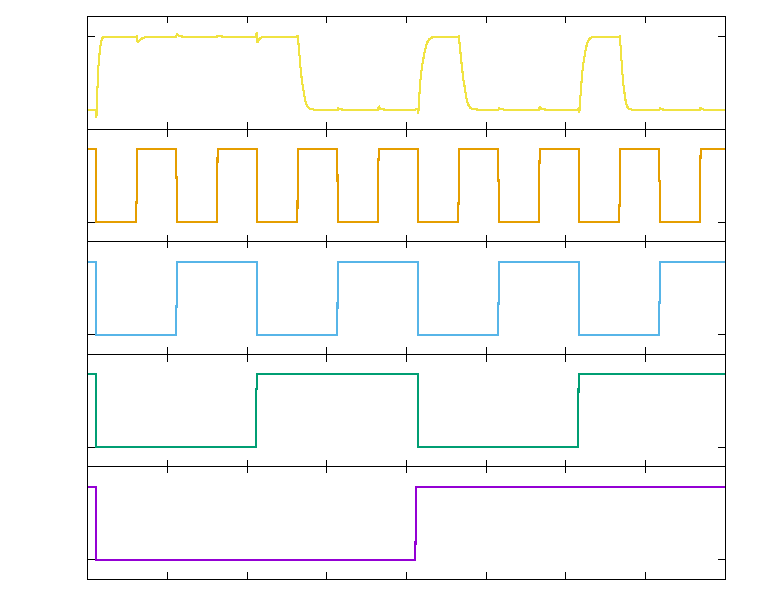
\includegraphics{oai_func}}%
    \gplfronttext
  \end{picture}%
\endgroup

    \endgroup
    \caption{Waveform plots of the output of an X4 inverter driving different amounts of load inverters.}
    \label{oai_func}
\end{figure}
\begin{figure}[htb]
    \centering
    \begingroup
    \fontsize{8pt}{8pt}\selectfont
    % GNUPLOT: LaTeX picture with Postscript
\begingroup
  \makeatletter
  \providecommand\color[2][]{%
    \GenericError{(gnuplot) \space\space\space\@spaces}{%
      Package color not loaded in conjunction with
      terminal option `colourtext'%
    }{See the gnuplot documentation for explanation.%
    }{Either use 'blacktext' in gnuplot or load the package
      color.sty in LaTeX.}%
    \renewcommand\color[2][]{}%
  }%
  \providecommand\includegraphics[2][]{%
    \GenericError{(gnuplot) \space\space\space\@spaces}{%
      Package graphicx or graphics not loaded%
    }{See the gnuplot documentation for explanation.%
    }{The gnuplot epslatex terminal needs graphicx.sty or graphics.sty.}%
    \renewcommand\includegraphics[2][]{}%
  }%
  \providecommand\rotatebox[2]{#2}%
  \@ifundefined{ifGPcolor}{%
    \newif\ifGPcolor
    \GPcolortrue
  }{}%
  \@ifundefined{ifGPblacktext}{%
    \newif\ifGPblacktext
    \GPblacktextfalse
  }{}%
  % define a \g@addto@macro without @ in the name:
  \let\gplgaddtomacro\g@addto@macro
  % define empty templates for all commands taking text:
  \gdef\gplbacktext{}%
  \gdef\gplfronttext{}%
  \makeatother
  \ifGPblacktext
    % no textcolor at all
    \def\colorrgb#1{}%
    \def\colorgray#1{}%
  \else
    % gray or color?
    \ifGPcolor
      \def\colorrgb#1{\color[rgb]{#1}}%
      \def\colorgray#1{\color[gray]{#1}}%
      \expandafter\def\csname LTw\endcsname{\color{white}}%
      \expandafter\def\csname LTb\endcsname{\color{black}}%
      \expandafter\def\csname LTa\endcsname{\color{black}}%
      \expandafter\def\csname LT0\endcsname{\color[rgb]{1,0,0}}%
      \expandafter\def\csname LT1\endcsname{\color[rgb]{0,1,0}}%
      \expandafter\def\csname LT2\endcsname{\color[rgb]{0,0,1}}%
      \expandafter\def\csname LT3\endcsname{\color[rgb]{1,0,1}}%
      \expandafter\def\csname LT4\endcsname{\color[rgb]{0,1,1}}%
      \expandafter\def\csname LT5\endcsname{\color[rgb]{1,1,0}}%
      \expandafter\def\csname LT6\endcsname{\color[rgb]{0,0,0}}%
      \expandafter\def\csname LT7\endcsname{\color[rgb]{1,0.3,0}}%
      \expandafter\def\csname LT8\endcsname{\color[rgb]{0.5,0.5,0.5}}%
    \else
      % gray
      \def\colorrgb#1{\color{black}}%
      \def\colorgray#1{\color[gray]{#1}}%
      \expandafter\def\csname LTw\endcsname{\color{white}}%
      \expandafter\def\csname LTb\endcsname{\color{black}}%
      \expandafter\def\csname LTa\endcsname{\color{black}}%
      \expandafter\def\csname LT0\endcsname{\color{black}}%
      \expandafter\def\csname LT1\endcsname{\color{black}}%
      \expandafter\def\csname LT2\endcsname{\color{black}}%
      \expandafter\def\csname LT3\endcsname{\color{black}}%
      \expandafter\def\csname LT4\endcsname{\color{black}}%
      \expandafter\def\csname LT5\endcsname{\color{black}}%
      \expandafter\def\csname LT6\endcsname{\color{black}}%
      \expandafter\def\csname LT7\endcsname{\color{black}}%
      \expandafter\def\csname LT8\endcsname{\color{black}}%
    \fi
  \fi
    \setlength{\unitlength}{0.0500bp}%
    \ifx\gptboxheight\undefined%
      \newlength{\gptboxheight}%
      \newlength{\gptboxwidth}%
      \newsavebox{\gptboxtext}%
    \fi%
    \setlength{\fboxrule}{0.5pt}%
    \setlength{\fboxsep}{1pt}%
\begin{picture}(7200.00,5400.00)%
    \gplgaddtomacro\gplbacktext{%
      \csname LTb\endcsname%%
      \put(682,704){\makebox(0,0)[r]{\strut{}$-1$}}%
      \put(682,1280){\makebox(0,0)[r]{\strut{}$0$}}%
      \put(682,1857){\makebox(0,0)[r]{\strut{}$1$}}%
      \put(682,2433){\makebox(0,0)[r]{\strut{}$2$}}%
      \put(682,3010){\makebox(0,0)[r]{\strut{}$3$}}%
      \put(682,3586){\makebox(0,0)[r]{\strut{}$4$}}%
      \put(682,4163){\makebox(0,0)[r]{\strut{}$5$}}%
      \put(682,4739){\makebox(0,0)[r]{\strut{}$6$}}%
      \put(814,484){\makebox(0,0){\strut{}$0$}}%
      \put(1563,484){\makebox(0,0){\strut{}$1\times10^{-9}$}}%
      \put(2311,484){\makebox(0,0){\strut{}$2\times10^{-9}$}}%
      \put(3060,484){\makebox(0,0){\strut{}$3\times10^{-9}$}}%
      \put(3809,484){\makebox(0,0){\strut{}$4\times10^{-9}$}}%
      \put(4557,484){\makebox(0,0){\strut{}$5\times10^{-9}$}}%
      \put(5306,484){\makebox(0,0){\strut{}$6\times10^{-9}$}}%
      \put(6054,484){\makebox(0,0){\strut{}$7\times10^{-9}$}}%
      \put(6803,484){\makebox(0,0){\strut{}$8\times10^{-9}$}}%
    }%
    \gplgaddtomacro\gplfronttext{%
      \csname LTb\endcsname%%
      \put(198,2721){\rotatebox{-270}{\makebox(0,0){\strut{}Voltage (V)}}}%
      \put(3808,154){\makebox(0,0){\strut{}Time (sec)}}%
      \put(3808,5069){\makebox(0,0){\strut{}Nor Simulation Plots}}%
      \csname LTb\endcsname%%
      \put(4076,2900){\makebox(0,0)[r]{\strut{}sA sch}}%
      \csname LTb\endcsname%%
      \put(4076,2680){\makebox(0,0)[r]{\strut{}sA ext}}%
      \csname LTb\endcsname%%
      \put(4076,2460){\makebox(0,0)[r]{\strut{}sB sch}}%
      \csname LTb\endcsname%%
      \put(4076,2240){\makebox(0,0)[r]{\strut{}sB ext}}%
    }%
    \gplbacktext
    \put(0,0){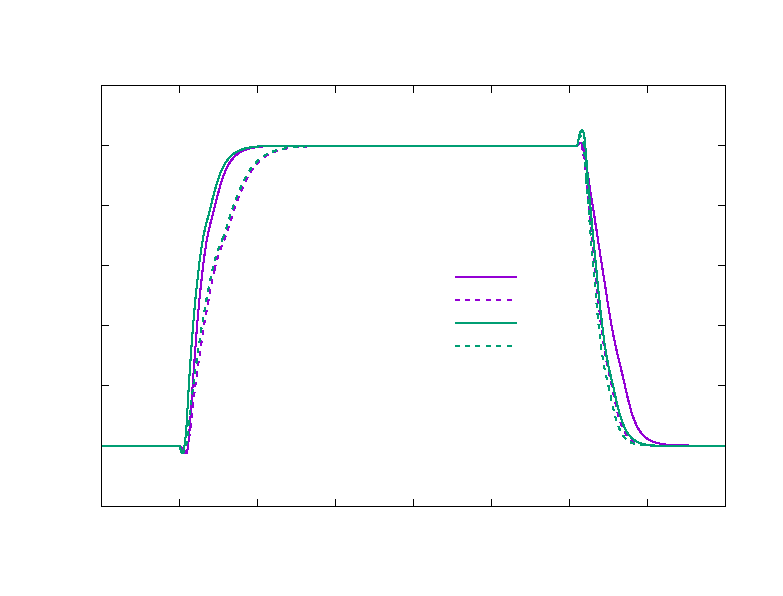
\includegraphics{nor}}%
    \gplfronttext
  \end{picture}%
\endgroup

    \endgroup
    \caption{Waveform plots of the output of an X4 inverter driving different amounts of load inverters.}
    \label{nor}
\end{figure}
\begin{figure}[htb]
    \centering
    \begingroup
    \fontsize{8pt}{8pt}\selectfont
    % GNUPLOT: LaTeX picture with Postscript
\begingroup
  \makeatletter
  \providecommand\color[2][]{%
    \GenericError{(gnuplot) \space\space\space\@spaces}{%
      Package color not loaded in conjunction with
      terminal option `colourtext'%
    }{See the gnuplot documentation for explanation.%
    }{Either use 'blacktext' in gnuplot or load the package
      color.sty in LaTeX.}%
    \renewcommand\color[2][]{}%
  }%
  \providecommand\includegraphics[2][]{%
    \GenericError{(gnuplot) \space\space\space\@spaces}{%
      Package graphicx or graphics not loaded%
    }{See the gnuplot documentation for explanation.%
    }{The gnuplot epslatex terminal needs graphicx.sty or graphics.sty.}%
    \renewcommand\includegraphics[2][]{}%
  }%
  \providecommand\rotatebox[2]{#2}%
  \@ifundefined{ifGPcolor}{%
    \newif\ifGPcolor
    \GPcolortrue
  }{}%
  \@ifundefined{ifGPblacktext}{%
    \newif\ifGPblacktext
    \GPblacktextfalse
  }{}%
  % define a \g@addto@macro without @ in the name:
  \let\gplgaddtomacro\g@addto@macro
  % define empty templates for all commands taking text:
  \gdef\gplbacktext{}%
  \gdef\gplfronttext{}%
  \makeatother
  \ifGPblacktext
    % no textcolor at all
    \def\colorrgb#1{}%
    \def\colorgray#1{}%
  \else
    % gray or color?
    \ifGPcolor
      \def\colorrgb#1{\color[rgb]{#1}}%
      \def\colorgray#1{\color[gray]{#1}}%
      \expandafter\def\csname LTw\endcsname{\color{white}}%
      \expandafter\def\csname LTb\endcsname{\color{black}}%
      \expandafter\def\csname LTa\endcsname{\color{black}}%
      \expandafter\def\csname LT0\endcsname{\color[rgb]{1,0,0}}%
      \expandafter\def\csname LT1\endcsname{\color[rgb]{0,1,0}}%
      \expandafter\def\csname LT2\endcsname{\color[rgb]{0,0,1}}%
      \expandafter\def\csname LT3\endcsname{\color[rgb]{1,0,1}}%
      \expandafter\def\csname LT4\endcsname{\color[rgb]{0,1,1}}%
      \expandafter\def\csname LT5\endcsname{\color[rgb]{1,1,0}}%
      \expandafter\def\csname LT6\endcsname{\color[rgb]{0,0,0}}%
      \expandafter\def\csname LT7\endcsname{\color[rgb]{1,0.3,0}}%
      \expandafter\def\csname LT8\endcsname{\color[rgb]{0.5,0.5,0.5}}%
    \else
      % gray
      \def\colorrgb#1{\color{black}}%
      \def\colorgray#1{\color[gray]{#1}}%
      \expandafter\def\csname LTw\endcsname{\color{white}}%
      \expandafter\def\csname LTb\endcsname{\color{black}}%
      \expandafter\def\csname LTa\endcsname{\color{black}}%
      \expandafter\def\csname LT0\endcsname{\color{black}}%
      \expandafter\def\csname LT1\endcsname{\color{black}}%
      \expandafter\def\csname LT2\endcsname{\color{black}}%
      \expandafter\def\csname LT3\endcsname{\color{black}}%
      \expandafter\def\csname LT4\endcsname{\color{black}}%
      \expandafter\def\csname LT5\endcsname{\color{black}}%
      \expandafter\def\csname LT6\endcsname{\color{black}}%
      \expandafter\def\csname LT7\endcsname{\color{black}}%
      \expandafter\def\csname LT8\endcsname{\color{black}}%
    \fi
  \fi
    \setlength{\unitlength}{0.0500bp}%
    \ifx\gptboxheight\undefined%
      \newlength{\gptboxheight}%
      \newlength{\gptboxwidth}%
      \newsavebox{\gptboxtext}%
    \fi%
    \setlength{\fboxrule}{0.5pt}%
    \setlength{\fboxsep}{1pt}%
\begin{picture}(7200.00,5400.00)%
    \gplgaddtomacro\gplbacktext{%
      \csname LTb\endcsname%%
      \put(682,704){\makebox(0,0)[r]{\strut{}$-1$}}%
      \put(682,1280){\makebox(0,0)[r]{\strut{}$0$}}%
      \put(682,1857){\makebox(0,0)[r]{\strut{}$1$}}%
      \put(682,2433){\makebox(0,0)[r]{\strut{}$2$}}%
      \put(682,3010){\makebox(0,0)[r]{\strut{}$3$}}%
      \put(682,3586){\makebox(0,0)[r]{\strut{}$4$}}%
      \put(682,4163){\makebox(0,0)[r]{\strut{}$5$}}%
      \put(682,4739){\makebox(0,0)[r]{\strut{}$6$}}%
      \put(814,484){\makebox(0,0){\strut{}$0$}}%
      \put(1563,484){\makebox(0,0){\strut{}$1\times10^{-9}$}}%
      \put(2311,484){\makebox(0,0){\strut{}$2\times10^{-9}$}}%
      \put(3060,484){\makebox(0,0){\strut{}$3\times10^{-9}$}}%
      \put(3809,484){\makebox(0,0){\strut{}$4\times10^{-9}$}}%
      \put(4557,484){\makebox(0,0){\strut{}$5\times10^{-9}$}}%
      \put(5306,484){\makebox(0,0){\strut{}$6\times10^{-9}$}}%
      \put(6054,484){\makebox(0,0){\strut{}$7\times10^{-9}$}}%
      \put(6803,484){\makebox(0,0){\strut{}$8\times10^{-9}$}}%
    }%
    \gplgaddtomacro\gplfronttext{%
      \csname LTb\endcsname%%
      \put(198,2721){\rotatebox{-270}{\makebox(0,0){\strut{}Voltage (V)}}}%
      \put(3808,154){\makebox(0,0){\strut{}Time (sec)}}%
      \put(3808,5069){\makebox(0,0){\strut{}Output Voltage vs. Time of Nand Gate with Differing Loads and Square Wave Input}}%
      \csname LTb\endcsname%%
      \put(5031,4566){\makebox(0,0)[r]{\strut{}1 Load Inverter Switch A}}%
      \csname LTb\endcsname%%
      \put(5031,4346){\makebox(0,0)[r]{\strut{}1 Load Inverter Switch B}}%
      \csname LTb\endcsname%%
      \put(5031,4126){\makebox(0,0)[r]{\strut{}2 Load Inverters Switch A}}%
      \csname LTb\endcsname%%
      \put(5031,3906){\makebox(0,0)[r]{\strut{}2 Load Inverters Switch B}}%
      \csname LTb\endcsname%%
      \put(5031,3686){\makebox(0,0)[r]{\strut{}4 Load Inverters Switch A}}%
      \csname LTb\endcsname%%
      \put(5031,3466){\makebox(0,0)[r]{\strut{}4 Load Inverters Switch B}}%
    }%
    \gplbacktext
    \put(0,0){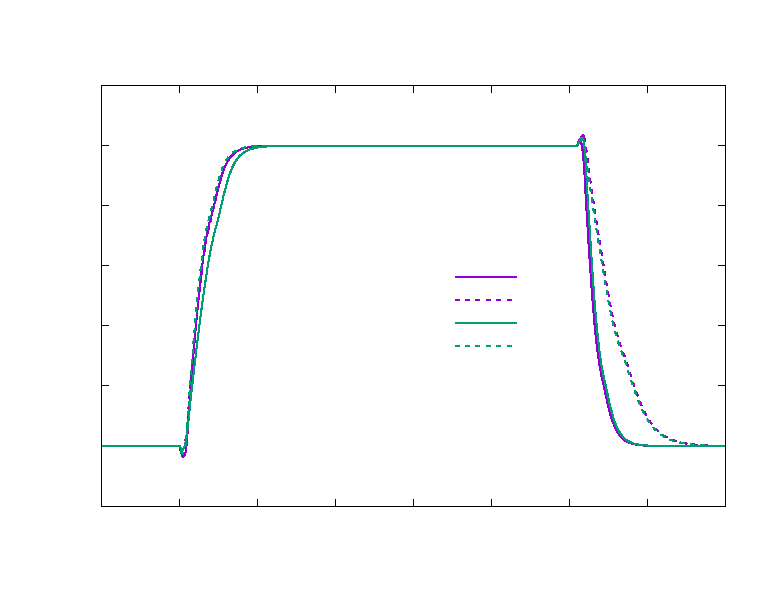
\includegraphics{nand}}%
    \gplfronttext
  \end{picture}%
\endgroup

    \endgroup
    \caption{Waveform plots of the output of an X4 inverter driving different amounts of load inverters.}
    \label{nand}
\end{figure}
\begin{figure}[htb]
    \centering
    \begingroup
    \fontsize{8pt}{8pt}\selectfont
    % GNUPLOT: LaTeX picture with Postscript
\begingroup
  \makeatletter
  \providecommand\color[2][]{%
    \GenericError{(gnuplot) \space\space\space\@spaces}{%
      Package color not loaded in conjunction with
      terminal option `colourtext'%
    }{See the gnuplot documentation for explanation.%
    }{Either use 'blacktext' in gnuplot or load the package
      color.sty in LaTeX.}%
    \renewcommand\color[2][]{}%
  }%
  \providecommand\includegraphics[2][]{%
    \GenericError{(gnuplot) \space\space\space\@spaces}{%
      Package graphicx or graphics not loaded%
    }{See the gnuplot documentation for explanation.%
    }{The gnuplot epslatex terminal needs graphicx.sty or graphics.sty.}%
    \renewcommand\includegraphics[2][]{}%
  }%
  \providecommand\rotatebox[2]{#2}%
  \@ifundefined{ifGPcolor}{%
    \newif\ifGPcolor
    \GPcolortrue
  }{}%
  \@ifundefined{ifGPblacktext}{%
    \newif\ifGPblacktext
    \GPblacktextfalse
  }{}%
  % define a \g@addto@macro without @ in the name:
  \let\gplgaddtomacro\g@addto@macro
  % define empty templates for all commands taking text:
  \gdef\gplbacktext{}%
  \gdef\gplfronttext{}%
  \makeatother
  \ifGPblacktext
    % no textcolor at all
    \def\colorrgb#1{}%
    \def\colorgray#1{}%
  \else
    % gray or color?
    \ifGPcolor
      \def\colorrgb#1{\color[rgb]{#1}}%
      \def\colorgray#1{\color[gray]{#1}}%
      \expandafter\def\csname LTw\endcsname{\color{white}}%
      \expandafter\def\csname LTb\endcsname{\color{black}}%
      \expandafter\def\csname LTa\endcsname{\color{black}}%
      \expandafter\def\csname LT0\endcsname{\color[rgb]{1,0,0}}%
      \expandafter\def\csname LT1\endcsname{\color[rgb]{0,1,0}}%
      \expandafter\def\csname LT2\endcsname{\color[rgb]{0,0,1}}%
      \expandafter\def\csname LT3\endcsname{\color[rgb]{1,0,1}}%
      \expandafter\def\csname LT4\endcsname{\color[rgb]{0,1,1}}%
      \expandafter\def\csname LT5\endcsname{\color[rgb]{1,1,0}}%
      \expandafter\def\csname LT6\endcsname{\color[rgb]{0,0,0}}%
      \expandafter\def\csname LT7\endcsname{\color[rgb]{1,0.3,0}}%
      \expandafter\def\csname LT8\endcsname{\color[rgb]{0.5,0.5,0.5}}%
    \else
      % gray
      \def\colorrgb#1{\color{black}}%
      \def\colorgray#1{\color[gray]{#1}}%
      \expandafter\def\csname LTw\endcsname{\color{white}}%
      \expandafter\def\csname LTb\endcsname{\color{black}}%
      \expandafter\def\csname LTa\endcsname{\color{black}}%
      \expandafter\def\csname LT0\endcsname{\color{black}}%
      \expandafter\def\csname LT1\endcsname{\color{black}}%
      \expandafter\def\csname LT2\endcsname{\color{black}}%
      \expandafter\def\csname LT3\endcsname{\color{black}}%
      \expandafter\def\csname LT4\endcsname{\color{black}}%
      \expandafter\def\csname LT5\endcsname{\color{black}}%
      \expandafter\def\csname LT6\endcsname{\color{black}}%
      \expandafter\def\csname LT7\endcsname{\color{black}}%
      \expandafter\def\csname LT8\endcsname{\color{black}}%
    \fi
  \fi
    \setlength{\unitlength}{0.0500bp}%
    \ifx\gptboxheight\undefined%
      \newlength{\gptboxheight}%
      \newlength{\gptboxwidth}%
      \newsavebox{\gptboxtext}%
    \fi%
    \setlength{\fboxrule}{0.5pt}%
    \setlength{\fboxsep}{1pt}%
\begin{picture}(7200.00,5400.00)%
    \gplgaddtomacro\gplbacktext{%
      \csname LTb\endcsname%%
      \put(682,704){\makebox(0,0)[r]{\strut{}$-1$}}%
      \put(682,1280){\makebox(0,0)[r]{\strut{}$0$}}%
      \put(682,1857){\makebox(0,0)[r]{\strut{}$1$}}%
      \put(682,2433){\makebox(0,0)[r]{\strut{}$2$}}%
      \put(682,3010){\makebox(0,0)[r]{\strut{}$3$}}%
      \put(682,3586){\makebox(0,0)[r]{\strut{}$4$}}%
      \put(682,4163){\makebox(0,0)[r]{\strut{}$5$}}%
      \put(682,4739){\makebox(0,0)[r]{\strut{}$6$}}%
      \put(814,484){\makebox(0,0){\strut{}$0$}}%
      \put(1563,484){\makebox(0,0){\strut{}$1\times10^{-9}$}}%
      \put(2311,484){\makebox(0,0){\strut{}$2\times10^{-9}$}}%
      \put(3060,484){\makebox(0,0){\strut{}$3\times10^{-9}$}}%
      \put(3809,484){\makebox(0,0){\strut{}$4\times10^{-9}$}}%
      \put(4557,484){\makebox(0,0){\strut{}$5\times10^{-9}$}}%
      \put(5306,484){\makebox(0,0){\strut{}$6\times10^{-9}$}}%
      \put(6054,484){\makebox(0,0){\strut{}$7\times10^{-9}$}}%
      \put(6803,484){\makebox(0,0){\strut{}$8\times10^{-9}$}}%
    }%
    \gplgaddtomacro\gplfronttext{%
      \csname LTb\endcsname%%
      \put(198,2721){\rotatebox{-270}{\makebox(0,0){\strut{}Voltage (V)}}}%
      \put(3808,154){\makebox(0,0){\strut{}Time (sec)}}%
      \put(3808,5069){\makebox(0,0){\strut{}OAI Simulation Plots}}%
      \csname LTb\endcsname%%
      \put(4076,2900){\makebox(0,0)[r]{\strut{}sA sch}}%
      \csname LTb\endcsname%%
      \put(4076,2680){\makebox(0,0)[r]{\strut{}sA ext}}%
      \csname LTb\endcsname%%
      \put(4076,2460){\makebox(0,0)[r]{\strut{}sB sch}}%
      \csname LTb\endcsname%%
      \put(4076,2240){\makebox(0,0)[r]{\strut{}sB ext}}%
      \csname LTb\endcsname%%
      \put(4076,2020){\makebox(0,0)[r]{\strut{}sC sch}}%
      \csname LTb\endcsname%%
      \put(4076,1800){\makebox(0,0)[r]{\strut{}sC ext}}%
      \csname LTb\endcsname%%
      \put(4076,1580){\makebox(0,0)[r]{\strut{}sD sch}}%
      \csname LTb\endcsname%%
      \put(4076,1360){\makebox(0,0)[r]{\strut{}sD ext}}%
    }%
    \gplbacktext
    \put(0,0){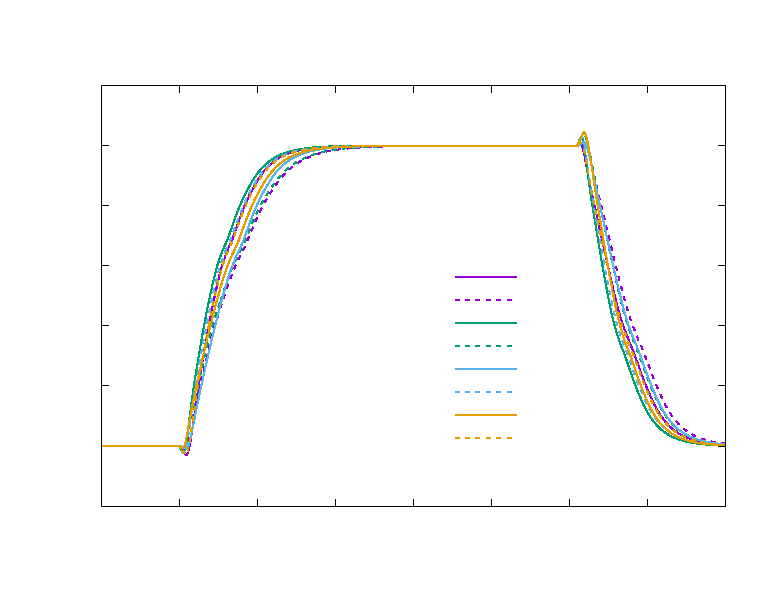
\includegraphics{oai}}%
    \gplfronttext
  \end{picture}%
\endgroup

    \endgroup
    \caption{Waveform plots of the output of an X4 inverter driving different amounts of load inverters.}
    \label{oai}
\end{figure}
\begin{figure}[htb]
    \centering
    \begingroup
    \fontsize{8pt}{8pt}\selectfont
    % GNUPLOT: LaTeX picture with Postscript
\begingroup
  \makeatletter
  \providecommand\color[2][]{%
    \GenericError{(gnuplot) \space\space\space\@spaces}{%
      Package color not loaded in conjunction with
      terminal option `colourtext'%
    }{See the gnuplot documentation for explanation.%
    }{Either use 'blacktext' in gnuplot or load the package
      color.sty in LaTeX.}%
    \renewcommand\color[2][]{}%
  }%
  \providecommand\includegraphics[2][]{%
    \GenericError{(gnuplot) \space\space\space\@spaces}{%
      Package graphicx or graphics not loaded%
    }{See the gnuplot documentation for explanation.%
    }{The gnuplot epslatex terminal needs graphicx.sty or graphics.sty.}%
    \renewcommand\includegraphics[2][]{}%
  }%
  \providecommand\rotatebox[2]{#2}%
  \@ifundefined{ifGPcolor}{%
    \newif\ifGPcolor
    \GPcolortrue
  }{}%
  \@ifundefined{ifGPblacktext}{%
    \newif\ifGPblacktext
    \GPblacktextfalse
  }{}%
  % define a \g@addto@macro without @ in the name:
  \let\gplgaddtomacro\g@addto@macro
  % define empty templates for all commands taking text:
  \gdef\gplbacktext{}%
  \gdef\gplfronttext{}%
  \makeatother
  \ifGPblacktext
    % no textcolor at all
    \def\colorrgb#1{}%
    \def\colorgray#1{}%
  \else
    % gray or color?
    \ifGPcolor
      \def\colorrgb#1{\color[rgb]{#1}}%
      \def\colorgray#1{\color[gray]{#1}}%
      \expandafter\def\csname LTw\endcsname{\color{white}}%
      \expandafter\def\csname LTb\endcsname{\color{black}}%
      \expandafter\def\csname LTa\endcsname{\color{black}}%
      \expandafter\def\csname LT0\endcsname{\color[rgb]{1,0,0}}%
      \expandafter\def\csname LT1\endcsname{\color[rgb]{0,1,0}}%
      \expandafter\def\csname LT2\endcsname{\color[rgb]{0,0,1}}%
      \expandafter\def\csname LT3\endcsname{\color[rgb]{1,0,1}}%
      \expandafter\def\csname LT4\endcsname{\color[rgb]{0,1,1}}%
      \expandafter\def\csname LT5\endcsname{\color[rgb]{1,1,0}}%
      \expandafter\def\csname LT6\endcsname{\color[rgb]{0,0,0}}%
      \expandafter\def\csname LT7\endcsname{\color[rgb]{1,0.3,0}}%
      \expandafter\def\csname LT8\endcsname{\color[rgb]{0.5,0.5,0.5}}%
    \else
      % gray
      \def\colorrgb#1{\color{black}}%
      \def\colorgray#1{\color[gray]{#1}}%
      \expandafter\def\csname LTw\endcsname{\color{white}}%
      \expandafter\def\csname LTb\endcsname{\color{black}}%
      \expandafter\def\csname LTa\endcsname{\color{black}}%
      \expandafter\def\csname LT0\endcsname{\color{black}}%
      \expandafter\def\csname LT1\endcsname{\color{black}}%
      \expandafter\def\csname LT2\endcsname{\color{black}}%
      \expandafter\def\csname LT3\endcsname{\color{black}}%
      \expandafter\def\csname LT4\endcsname{\color{black}}%
      \expandafter\def\csname LT5\endcsname{\color{black}}%
      \expandafter\def\csname LT6\endcsname{\color{black}}%
      \expandafter\def\csname LT7\endcsname{\color{black}}%
      \expandafter\def\csname LT8\endcsname{\color{black}}%
    \fi
  \fi
    \setlength{\unitlength}{0.0500bp}%
    \ifx\gptboxheight\undefined%
      \newlength{\gptboxheight}%
      \newlength{\gptboxwidth}%
      \newsavebox{\gptboxtext}%
    \fi%
    \setlength{\fboxrule}{0.5pt}%
    \setlength{\fboxsep}{1pt}%
\begin{picture}(7200.00,5400.00)%
    \gplgaddtomacro\gplbacktext{%
      \csname LTb\endcsname%%
      \put(682,704){\makebox(0,0)[r]{\strut{}$-1$}}%
      \put(682,1280){\makebox(0,0)[r]{\strut{}$0$}}%
      \put(682,1857){\makebox(0,0)[r]{\strut{}$1$}}%
      \put(682,2433){\makebox(0,0)[r]{\strut{}$2$}}%
      \put(682,3010){\makebox(0,0)[r]{\strut{}$3$}}%
      \put(682,3586){\makebox(0,0)[r]{\strut{}$4$}}%
      \put(682,4163){\makebox(0,0)[r]{\strut{}$5$}}%
      \put(682,4739){\makebox(0,0)[r]{\strut{}$6$}}%
      \put(814,484){\makebox(0,0){\strut{}$0$}}%
      \put(1563,484){\makebox(0,0){\strut{}$1\times10^{-9}$}}%
      \put(2311,484){\makebox(0,0){\strut{}$2\times10^{-9}$}}%
      \put(3060,484){\makebox(0,0){\strut{}$3\times10^{-9}$}}%
      \put(3809,484){\makebox(0,0){\strut{}$4\times10^{-9}$}}%
      \put(4557,484){\makebox(0,0){\strut{}$5\times10^{-9}$}}%
      \put(5306,484){\makebox(0,0){\strut{}$6\times10^{-9}$}}%
      \put(6054,484){\makebox(0,0){\strut{}$7\times10^{-9}$}}%
      \put(6803,484){\makebox(0,0){\strut{}$8\times10^{-9}$}}%
    }%
    \gplgaddtomacro\gplfronttext{%
      \csname LTb\endcsname%%
      \put(198,2721){\rotatebox{-270}{\makebox(0,0){\strut{}Voltage (V)}}}%
      \put(3808,154){\makebox(0,0){\strut{}Time (sec)}}%
      \put(3808,5069){\makebox(0,0){\strut{}AOI Simulation Plots}}%
      \csname LTb\endcsname%%
      \put(4076,2900){\makebox(0,0)[r]{\strut{}sA sch}}%
      \csname LTb\endcsname%%
      \put(4076,2680){\makebox(0,0)[r]{\strut{}sA ext}}%
      \csname LTb\endcsname%%
      \put(4076,2460){\makebox(0,0)[r]{\strut{}sB sch}}%
      \csname LTb\endcsname%%
      \put(4076,2240){\makebox(0,0)[r]{\strut{}sB ext}}%
      \csname LTb\endcsname%%
      \put(4076,2020){\makebox(0,0)[r]{\strut{}sC sch}}%
      \csname LTb\endcsname%%
      \put(4076,1800){\makebox(0,0)[r]{\strut{}sC ext}}%
      \csname LTb\endcsname%%
      \put(4076,1580){\makebox(0,0)[r]{\strut{}sD sch}}%
      \csname LTb\endcsname%%
      \put(4076,1360){\makebox(0,0)[r]{\strut{}sD ext}}%
    }%
    \gplbacktext
    \put(0,0){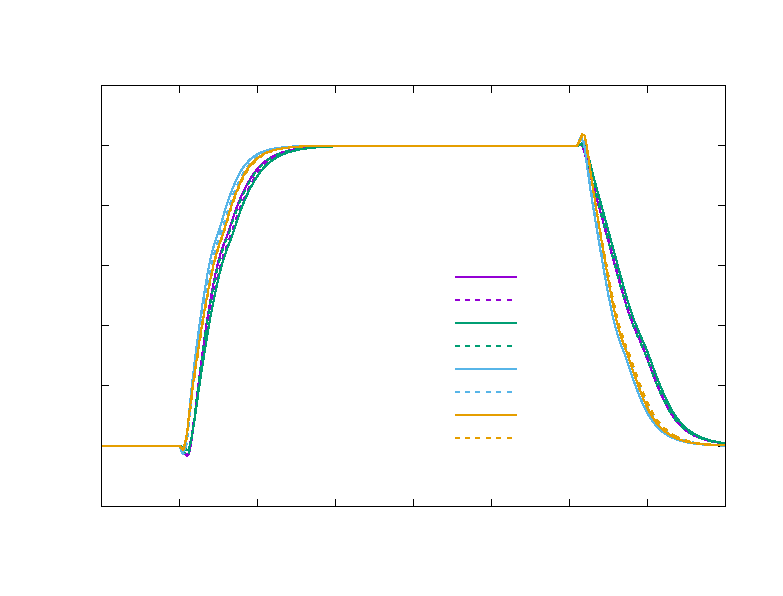
\includegraphics{aoi}}%
    \gplfronttext
  \end{picture}%
\endgroup

    \endgroup
    \caption{Waveform plots of the output of an X4 inverter driving different amounts of load inverters.}
    \label{aoi}
\end{figure}
\begin{figure}[htb]
    \centering
    \begingroup
    \fontsize{8pt}{8pt}\selectfont
    % GNUPLOT: LaTeX picture with Postscript
\begingroup
  \makeatletter
  \providecommand\color[2][]{%
    \GenericError{(gnuplot) \space\space\space\@spaces}{%
      Package color not loaded in conjunction with
      terminal option `colourtext'%
    }{See the gnuplot documentation for explanation.%
    }{Either use 'blacktext' in gnuplot or load the package
      color.sty in LaTeX.}%
    \renewcommand\color[2][]{}%
  }%
  \providecommand\includegraphics[2][]{%
    \GenericError{(gnuplot) \space\space\space\@spaces}{%
      Package graphicx or graphics not loaded%
    }{See the gnuplot documentation for explanation.%
    }{The gnuplot epslatex terminal needs graphicx.sty or graphics.sty.}%
    \renewcommand\includegraphics[2][]{}%
  }%
  \providecommand\rotatebox[2]{#2}%
  \@ifundefined{ifGPcolor}{%
    \newif\ifGPcolor
    \GPcolortrue
  }{}%
  \@ifundefined{ifGPblacktext}{%
    \newif\ifGPblacktext
    \GPblacktextfalse
  }{}%
  % define a \g@addto@macro without @ in the name:
  \let\gplgaddtomacro\g@addto@macro
  % define empty templates for all commands taking text:
  \gdef\gplbacktext{}%
  \gdef\gplfronttext{}%
  \makeatother
  \ifGPblacktext
    % no textcolor at all
    \def\colorrgb#1{}%
    \def\colorgray#1{}%
  \else
    % gray or color?
    \ifGPcolor
      \def\colorrgb#1{\color[rgb]{#1}}%
      \def\colorgray#1{\color[gray]{#1}}%
      \expandafter\def\csname LTw\endcsname{\color{white}}%
      \expandafter\def\csname LTb\endcsname{\color{black}}%
      \expandafter\def\csname LTa\endcsname{\color{black}}%
      \expandafter\def\csname LT0\endcsname{\color[rgb]{1,0,0}}%
      \expandafter\def\csname LT1\endcsname{\color[rgb]{0,1,0}}%
      \expandafter\def\csname LT2\endcsname{\color[rgb]{0,0,1}}%
      \expandafter\def\csname LT3\endcsname{\color[rgb]{1,0,1}}%
      \expandafter\def\csname LT4\endcsname{\color[rgb]{0,1,1}}%
      \expandafter\def\csname LT5\endcsname{\color[rgb]{1,1,0}}%
      \expandafter\def\csname LT6\endcsname{\color[rgb]{0,0,0}}%
      \expandafter\def\csname LT7\endcsname{\color[rgb]{1,0.3,0}}%
      \expandafter\def\csname LT8\endcsname{\color[rgb]{0.5,0.5,0.5}}%
    \else
      % gray
      \def\colorrgb#1{\color{black}}%
      \def\colorgray#1{\color[gray]{#1}}%
      \expandafter\def\csname LTw\endcsname{\color{white}}%
      \expandafter\def\csname LTb\endcsname{\color{black}}%
      \expandafter\def\csname LTa\endcsname{\color{black}}%
      \expandafter\def\csname LT0\endcsname{\color{black}}%
      \expandafter\def\csname LT1\endcsname{\color{black}}%
      \expandafter\def\csname LT2\endcsname{\color{black}}%
      \expandafter\def\csname LT3\endcsname{\color{black}}%
      \expandafter\def\csname LT4\endcsname{\color{black}}%
      \expandafter\def\csname LT5\endcsname{\color{black}}%
      \expandafter\def\csname LT6\endcsname{\color{black}}%
      \expandafter\def\csname LT7\endcsname{\color{black}}%
      \expandafter\def\csname LT8\endcsname{\color{black}}%
    \fi
  \fi
    \setlength{\unitlength}{0.0500bp}%
    \ifx\gptboxheight\undefined%
      \newlength{\gptboxheight}%
      \newlength{\gptboxwidth}%
      \newsavebox{\gptboxtext}%
    \fi%
    \setlength{\fboxrule}{0.5pt}%
    \setlength{\fboxsep}{1pt}%
\begin{picture}(7200.00,5400.00)%
    \gplgaddtomacro\gplbacktext{%
      \csname LTb\endcsname%%
      \put(682,704){\makebox(0,0)[r]{\strut{}$-1$}}%
      \put(682,1280){\makebox(0,0)[r]{\strut{}$0$}}%
      \put(682,1857){\makebox(0,0)[r]{\strut{}$1$}}%
      \put(682,2433){\makebox(0,0)[r]{\strut{}$2$}}%
      \put(682,3010){\makebox(0,0)[r]{\strut{}$3$}}%
      \put(682,3586){\makebox(0,0)[r]{\strut{}$4$}}%
      \put(682,4163){\makebox(0,0)[r]{\strut{}$5$}}%
      \put(682,4739){\makebox(0,0)[r]{\strut{}$6$}}%
      \put(814,484){\makebox(0,0){\strut{}$0$}}%
      \put(1563,484){\makebox(0,0){\strut{}$1\times10^{-9}$}}%
      \put(2311,484){\makebox(0,0){\strut{}$2\times10^{-9}$}}%
      \put(3060,484){\makebox(0,0){\strut{}$3\times10^{-9}$}}%
      \put(3809,484){\makebox(0,0){\strut{}$4\times10^{-9}$}}%
      \put(4557,484){\makebox(0,0){\strut{}$5\times10^{-9}$}}%
      \put(5306,484){\makebox(0,0){\strut{}$6\times10^{-9}$}}%
      \put(6054,484){\makebox(0,0){\strut{}$7\times10^{-9}$}}%
      \put(6803,484){\makebox(0,0){\strut{}$8\times10^{-9}$}}%
    }%
    \gplgaddtomacro\gplfronttext{%
      \csname LTb\endcsname%%
      \put(198,2721){\rotatebox{-270}{\makebox(0,0){\strut{}Voltage (V)}}}%
      \put(3808,154){\makebox(0,0){\strut{}Time (sec)}}%
      \put(3808,5069){\makebox(0,0){\strut{}Output of Extracted View Sim vs Schematic View Sim}}%
      \csname LTb\endcsname%%
      \put(4076,2900){\makebox(0,0)[r]{\strut{}Schematic Sim}}%
      \csname LTb\endcsname%%
      \put(4076,2680){\makebox(0,0)[r]{\strut{}Extracted Sim}}%
    }%
    \gplbacktext
    \put(0,0){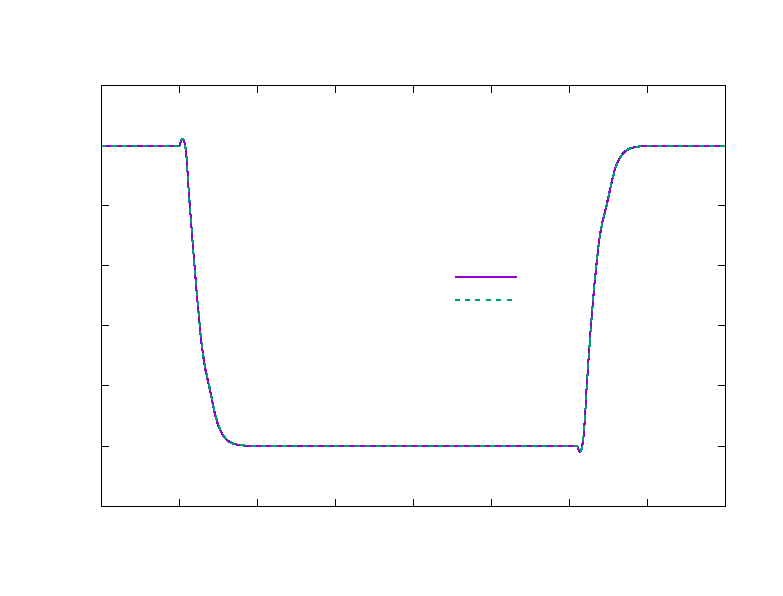
\includegraphics{INVx1}}%
    \gplfronttext
  \end{picture}%
\endgroup

    \endgroup
    \caption{Waveform plots of the output of an X4 inverter driving different amounts of load inverters.}
    \label{INVx1}
\end{figure}
\end{document}
